 %!TeX root = PHYS42 Lecture Notes.tex
\documentclass{article}
\usepackage[dvipsnames, svgnames, x11names]{xcolor}
\usepackage{tikz}
\usepackage{pgfplots}
\usepackage{pgfplotstable}
\usepackage{setspace}
\usepackage{units}
\usepackage{booktabs}
\usepackage{graphicx}
\usepackage{circuitikz}
\usepackage{multirow}
\usepackage{amsopn}
\usepackage{bbding}
\usepackage{amsmath}
\usepackage{hyperref}
\usepackage{cancel}
\usepackage{gensymb}
\usepackage[margin = 1.2in]{geometry}
\ctikzset{bipoles/thickness=1.2}

\newcommand{\midlabelline}[3]{
   \node (midlabel) at ($ (#1)!.5!(#2) $) {#3};
   \draw[latex-] (#1) --  (midlabel);
   \draw[-latex] (midlabel) -- (#2);
}

\AtBeginEnvironment{document}{\everymath{\displaystyle}}
\title{MATH 2 Lecture Notes}
\date{Tuesday, 14 January, 2025}
\author{Tejas Patel}
\begin{document}
\maketitle
\tableofcontents
\pagebreak
\section{Chapter 1}
\subsection{Terminology}
\textbf{Definition} A differential equation is an equation containing the derivatives or differentials 
of one or more dependent variables, with respect to one or more independent variables.\\
\textbf{$\cdot$} An Ordinary Differential Equation (ODE) involves only ordinary derivatives\\
\textbf{$\cdot$} A Partial Differential Equation (PDE) involves partial derivatives.\\
\textbf{Definition} The order of a DE is the order of the highest-order derivative that appears in the DE
\textbf{Notation} $F(x,y,\frac{dy}{dx}, \frac{d^2y}{dx^2})$\\
\textbf{Definition} A linear DE is any DE that can be written in form:\\
${\displaystyle a_{0}(x)y+a_{1}(x)y'+a_{2}(x)y''\cdots +a_{n}(x)y^{(n)}=b(x)}$\\
For a DE to be linear:
\begin{enumerate}
    \item Y and all of its derivatives much be of the 1st degree
    \item Any term that does not include y or any of its derivatives must be a function of x
\end{enumerate}

\subsection{Some Mathematical Models}
\subsubsection*{I. Free-falling body}
Goal: Find s(t). 
\\Set up a differential equation in S, model it, then solve
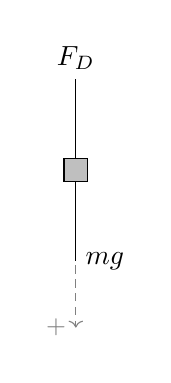
\begin{tikzpicture}[
    force/.style={>=latex,draw=blue,fill=blue},
    axis/.style={densely dashed,gray,font=\small},
    M/.style={rectangle,draw,fill=lightgray,minimum size=0.5cm,thin},
    m/.style={rectangle,draw=black,fill=lightgray,minimum size=0.3cm,thin},
    plane/.style={draw=black,fill=blue!10},
    string/.style={draw=red, thick},
    pulley/.style={thick},
]
\matrix[column sep=1cm] {
    \node[m] (m) {};

    \draw[axis,->] (m) -- ++(0,-2) node[left] {$+$};
    {[force,->]
    \draw (m.north) -- ++(0,1) node[above] {$F_D$};
        \draw (m.south) -- ++(0,-1) node[right] {$mg$};
    }
\\
};
\end{tikzpicture}\\
$ma=mg\\\frac{d^2s}{dt^2}=g\\v=\frac{ds}{dt}, g=\frac{dv}{dt}$\\
What if there is air resistance. Assume force scales linear with velocity
\\$\frac{dv}{dt}=g-\frac{kv}{m} \rightarrow \frac{dv}{dt}=g-\frac{k}{m}\cdot \frac{ds}{dt}$
\subsubsection*{II: Series Circuit}
\begin{circuitikz}
    \draw[line width=0.8]
     (2,7) to [sinusoidal voltage source, l_=$V_S$, i=$I$] (2,1)
     (2,7) to [resistor, l_=$R$] ++(6,0) to [inductor, l_=$L$] ++(0,-6) to [capacitor, l_=$C$] +(-6,0) ;
    \midlabelline{2,8}{8,8}{$V_R$}
    \midlabelline{9,7}{9,1}{$V_L$}
    \midlabelline{2,0}{8,0}{$V_C$}
\end{circuitikz}

Voltage drops:\\ $
V=L \frac{dI}{dt}, V=L \frac{d^2q}{dt^2}\\
V=IR, V= R \frac{dq}{dt}\\
V=\frac{q}{C}\\
E(t) = L \frac{d^2q}{dt^2}+ R \frac{dq}{dt} + \frac{q}{C}
$
\subsubsection*{III: Population Growth}
$P=P(t) =$ population at time t — use exponential model \\
$\frac{dp}{dt} \propto P \rightarrow \frac{dp}{dt} = kP \rightarrow = Ce^{kt}$ where C is the initial population
\subsubsection*{IV: Population Growth with Finite Capacity}
"Carrying Capacity" = N — uses the logistic growth model\\
$\frac{dp}{dt} \propto $ both P and amount to carrying capacity (N-P)\\
$\frac{dp}{dt}=kP(N-P)$
\subsubsection*{V: Chemical Reaction}
$A+B\rightarrow C$ Concentrations of A and B decreases by amount of C formed \\ 
Can we write DE governing the concentration of C x(t)? \\ 
The rate at which the reaaction takes place $\propto$ Product of the remaining concentrations of A and B
\\ $\alpha$ initial concentration of A
\\ $\beta$ initial concentration of B
\\ $\frac{dx}{dt} = k(\alpha - x)(\beta - x)$








\pagebreak
\section{Example Problems with Solutions}
\subsection{}
$\frac{dy}{dx}=y^2+2xy$
\end{document}